\section{Benchmark Construction}
\label{sec:benchmark}

\subsection{Data Source: Real User Interaction Traces}
\label{sec:data-source}
% \subsection{数据来源：真实用户交互轨迹}

Unlike synthetic benchmarks constructed by task authors, \bench{} is built from \emph{real user interaction traces}---actual multi-turn sessions where IC design engineers used a coding agent~\cite{cline2026} to solve design-flow problems in a production environment. We systematically scanned engineering workstations, identified sessions containing EDA-related tool interactions, and curated tasks from the most representative ones.
% 与由任务作者构造的合成基准不同，\bench{} 构建于"真实用户交互轨迹"之上——即 IC 设计工程师在生产环境中使用编程智能体解决设计流问题的真实多轮会话。我们系统性地扫描了工程工作站，识别出包含 EDA 相关工具交互的会话，并从中挑选最具代表性的部分整理为任务。

\textbf{Scan pipeline.} We grep session files for EDA-keyword matches (hspice, spectre, calibre, virtuoso, aether, innovus, pt\_shell, dc\_shell, netlist, schematic, etc.) and rank sessions by \emph{match-count} (mc)---the number of lines hitting any EDA keyword. A two-stage prefilter (rule-based + 0.8B LLM classifier) filters non-design-flow sessions (Q\&A, permission-denied, tool-not-found), with 0\% rejection rate on the mc $\geq 30$ pool---confirming that high-mc sessions are almost universally genuine EDA work.
% \textbf{扫描流程。} 我们对会话文件进行 EDA 关键词匹配（hspice、spectre、calibre、virtuoso、aether、innovus、pt\_shell、dc\_shell、netlist、schematic 等），并按"匹配计数"(mc)——命中任意 EDA 关键词的行数——对会话排序。一个两级预筛器（基于规则 + 0.8B LLM 分类器）过滤掉非设计流会话（问答、权限被拒、工具未找到），在 mc $\geq 30$ 池上拒绝率为 0\%——印证了高 mc 会话几乎全都是真实的 EDA 工作。

\textbf{Trace attribution.} Each task records \texttt{trace\_source} (host, user, session\_file, session\_msgs, real\_task\_summary), enabling trace-back to the original engineer's workflow. User identifiers are preserved (not hashed) for reproducibility, with only API keys/tokens masked.
% \textbf{轨迹溯源。} 每个任务记录 \texttt{trace\_source}（主机、用户、会话文件、会话消息数、真实任务摘要），可回溯至原始工程师的工作流。用户标识保留（不做哈希）以保证可复现性，仅对 API 密钥/令牌进行脱敏。

\subsection{Task Schema: The \mode{} Contract}
\label{sec:task-schema}
% \subsection{任务模式：\mode{} 契约}

All \Ntasks{} tasks follow a unified \mode{} contract (Table~\ref{tab:task-schema}):
% 所有 \Ntasks{} 个任务遵循统一的 \mode{} 契约（表~\ref{tab:task-schema}）：

\begin{itemize}
    \item \textbf{Prompt}: A natural-language task description derived from the real user's intent, reformulated to be self-contained (no assumed context from the original session).
    % \textbf{提示词}：源自真实用户意图的自然语言任务描述，改写为自包含形式（不依赖原始会话的上下文）。
    \item \textbf{Assets}: Input files (RTL fragments, simulation logs, technology files, spec documents) that the agent reads locally.
    % \textbf{附件}：智能体在本地读取的输入文件（RTL 片段、仿真日志、工艺文件、规格文档）。
    \item \textbf{Entry point}: \texttt{outputs/submit.zip}---the agent must write deliverable files under \texttt{outputs/} and the harness packages them into \texttt{submit.zip}.
    % \textbf{入口点}：\texttt{outputs/submit.zip}——智能体须将交付件写入 \texttt{outputs/}，由评测框架打包为 \texttt{submit.zip}。
    \item \textbf{Test}: A two-parameter check function \texttt{check(deliverable, workdir)} that unpacks the deliverable and runs $\geq 8$ assertions.
    % \textbf{测试}：一个双参判分函数 \texttt{check(deliverable, workdir)}，解包交付件并运行不少于 8 条断言。
    \item \textbf{No lang/host}: Unlike single-script benchmarks, the task does not specify a language or runtime---the agent must infer the appropriate tool chain from the task description.
    % \textbf{不指定语言/主机}：与单脚本基准不同，任务不指定编程语言或运行时——智能体须从任务描述自行推断合适的工具链。
\end{itemize}

\begin{table}[ht]
\centering
\small
\caption{Task schema comparison: single-script (EDA-Scripting-Bench) vs.\ \mode{} (\bench).}
% \caption{任务模式对比：单脚本（EDA-Scripting-Bench）vs.\ \mode{}（\bench）。}
\label{tab:task-schema}
\begin{tabularx}{\linewidth}{@{}lXX@{}}
\toprule
 & \textbf{Single-script} & \textbf{Design-flow (\bench)} \\
\midrule
Entry point & function return value & \texttt{outputs/\allowbreak submit.zip} \\
Tool interaction & single \texttt{run\_code} & multi-step MCP orchestration \\
Deliverable & one code file & multi-file package \\
Assertions & function-level & deliverable-level ($\geq 8$) \\
Lang/host specified & yes (pyAether/\allowbreak SKILL/\allowbreak Tcl) & no (agent infers) \\
Steps & 1--3 tool calls & 5--20+ tool calls \\
\bottomrule
\end{tabularx}
\end{table}

\subsection{Domain Coverage}
\label{sec:domain-coverage}
% \subsection{领域覆盖}

\bench{} spans 13 EDA design domains (Figure~\ref{fig:domain-distribution}), organized into four area groups:
% \bench{} 覆盖 13 个 EDA 设计领域（图~\ref{fig:domain-distribution}），按方向组织为四个领域组：
% 注：不再在正文写死的组内任务数——living build 每轮都在增长（2026-11-10: \Ntasks{}），
% 写死的组计数会立刻过期；精确的 shard 计数见附录~\ref{sec:benchmark-details}。

\begin{itemize}
    \item \textbf{Digital front}: digital, verification, pnr\_signoff, eda\_other
    % \textbf{数字前端}：digital、verification、pnr\_signoff、eda\_other
    \item \textbf{SPICE / characterization}: spice\_sim, characterization
    % \textbf{SPICE / 表征}：spice\_sim、characterization
    \item \textbf{Physical / layout}: physical\_verify, layout\_aether, layout\_virtuoso, pg\_layout
    % \textbf{物理 / 版图}：physical\_verify、layout\_aether、layout\_virtuoso、pg\_layout
    \item \textbf{Schematic / netlist / analog}: schematic\_netlist, waveform, analog\_context
    % \textbf{原理图 / 网表 / 模拟}：schematic\_netlist、waveform、analog\_context
\end{itemize}

The living benchmark currently holds \Ntasks{} curated cases (the \emph{Full set}); all results in
Sections~\ref{sec:experiments}--\ref{sec:analysis} are reported on a \emph{frozen
evaluation snapshot} of \Neval{} runs (2026-11-09), whose domain mix is shown in
Figure~\ref{fig:domain-distribution}. Freezing the snapshot is what makes the
per-domain table, the failure analysis and any future re-run comparable.
% 活基准当前含 \Ntasks{} 个已整理案例（\emph{Full 集}）；第~\ref{sec:experiments}--\ref{sec:analysis}~节的
% 全部结果都报告在一个 \emph{冻结的评测快照}（2026-11-09，\Neval{} 个 run）上，其领域构成见
% 图~\ref{fig:domain-distribution}。冻结快照是逐域表格、失败分析与将来重跑可比性的前提。

\textbf{Lite set.} To enable efficient daily evaluation and external reproduction,
we release a \emph{Lite set} of \LiteSet{} tasks selected from the Full set along
three dimensions: (i) \emph{domain balance}---stratified sampling across all 13
EDA domains so that no single domain exceeds 15\% of the Lite set; (ii)
\emph{difficulty calibration}---retaining tasks whose reference pass rate under
the frozen snapshot falls in the 5--25\% band, so that the Lite set is neither
trivially easy nor uniformly impossible; and (iii) \emph{releaseability}---tasks
whose underlying design assets have been approved for external publication are
prioritized, so that the Lite set can be fully released without confidentiality
constraints. The Lite set is intended as the default evaluation surface for new
agents; the Full set remains available for organizations that can access the
full asset inventory.
% \textbf{Lite 集}。为支持高效的日常评测与外部复现，我们从 Full 集中按三个维度筛选
% \LiteSet{} 个任务作为 \emph{Lite 集}：(i) 领域均衡——在 13 个 EDA 领域上分层抽样，
% 任一领域不超过 Lite 集的 15\%；(ii) 难度校准——保留冻结快照下参考通过率在 5--25\% 区间的任务，
% 使 Lite 集既非 trivial 也非 uniformly impossible；(iii) 可释放性——优先选择底座设计资产
% 已获对外发布批准的任务，使 Lite 集可在无保密约束下完整发布。Lite 集是新智能体评测的默认入口；
% Full 集仍可供能访问完整资产清单的组织使用。

The distribution reflects real engineering practice: schematic/netlist and SPICE simulation dominate (analog/mixed-signal design accounts for the largest share), while digital synthesis and PNR signoff are comparatively underrepresented---not because they are less important, but because digital engineers use coding agents less frequently (they work in IDEs and command-line flows). We revisit the implications of this imbalance in Section~\ref{sec:threats}.
% 该分布反映了真实工程实践：原理图/网表与 SPICE 仿真占主导（模拟/混合信号设计占比最大），而数字综合与 PNR 签核相对偏少——并非因为它们不重要，而是因为数字工程师较少使用编程智能体（他们多在 IDE 和命令行流程中工作）。我们在第~\ref{sec:threats}~节重新讨论这种失衡的影响。

\begin{figure}[ht]
\centering
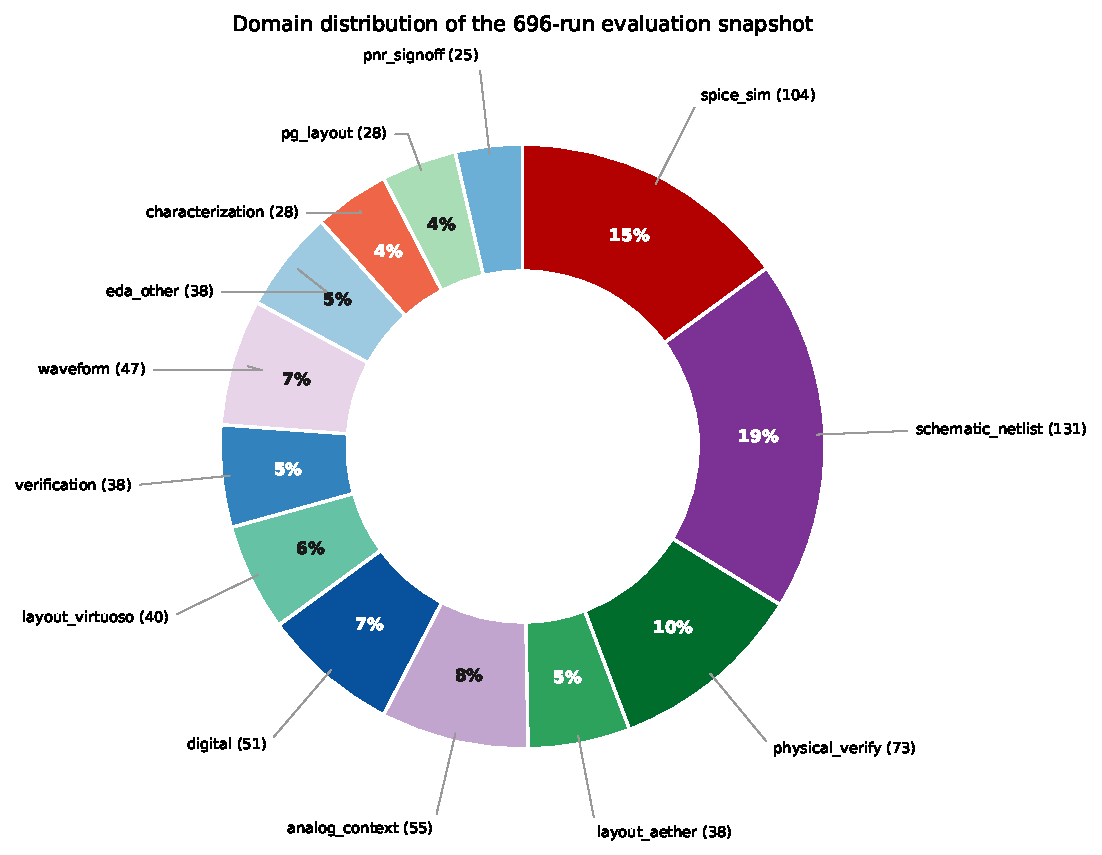
\includegraphics[width=\linewidth]{figures/domain_pie.pdf}
\caption{Domain distribution of the frozen \Neval{}-run evaluation snapshot across 13 EDA domains, colored by area group (counts include the 70 ERROR and 6 ABSENT runs of Table~\ref{tab:full-domain-results}). The donut layout keeps small slices legible; percentages are shown for slices $\geq 4\%$.}
% \caption{冻结的 \Neval{} 个 run 评测快照在 13 个 EDA 领域上的分布，按领域组着色（含表~\ref{tab:full-domain-results} 的 70 个 ERROR 与 6 个 ABSENT）。环形布局使小切片也可读；占比 $\geq 4\%$ 的切片显示百分比。}
\label{fig:domain-distribution}
\end{figure}

\subsection{Evaluation Metric and Protocol}
\label{sec:eval-protocol}
% \subsection{评测指标与协议}

\textbf{Pass@1.} One trace per task: the agent may iterate within the trace (multiple tool calls) but is never restarted. A 2400-second timeout per task. A task passes iff \emph{all} $k \geq 8$ assertions in the reference \texttt{check.py} hold.
% \textbf{Pass@1。} 每个任务一次轨迹：智能体可在该轨迹内迭代（多次工具调用），但不会被重启。每个任务超时 2400 秒。当且仅当参考 \texttt{check.py} 中所有 $k \geq 8$ 条断言全部成立时，该任务判为通过。

\textbf{Execution-based scoring.} The reference judge unpacks \texttt{submit.zip} into a fresh workdir and runs assertions against the deliverable, using only Python standard library (no EDA license required for judging). Each assertion is documented in the \texttt{test\_rationale} field as ``k assertions: (1), (2), ...'' for interpretability.
% \textbf{执行式判分。} 参考判分器将 \texttt{submit.zip} 解包到一个全新的工作目录，并针对交付件运行断言，仅使用 Python 标准库（判分无需 EDA 许可证）。每条断言以"k 条断言：(1)、(2)、……"的形式记录在 \texttt{test\_rationale} 字段中，便于可解释性。

The full evaluation harness---including the agent system, MCP bridge, anti-leakage hook, and judge implementation---is described in Section~\ref{sec:harness} (main text) and Appendix~\ref{sec:experimental-details} (implementation details).
% 完整的评测框架——包括智能体系统、MCP 网桥、防泄题钩子和判分器实现——在正文第~\ref{sec:harness}~节和附录~\ref{sec:experimental-details}~节（实现细节）中描述。
